\tikzset{external/export next=false}%
\begin{tikzpicture}
	\tikzstyle{every node}=[object, text width=6em]
	\tikzstyle{edge from parent}=[%
	draw,
	color=primary_inverse_fg,
	edge from parent path={(\tikzparentnode.south)-- +(0,-8pt)-| (\tikzchildnode)}
	]
	\node [text width=13em]{Predictors of the effect of mutations}[sibling distance=18em, level distance=4em]
	child {%
	node{Supervised}[sibling distance=8em, level distance=8em]
	child {%
	node {%
	\begin{minipage}{.6\textwidth}%
		Statistical model
	\end{minipage}%
	\begin{minipage}{.4\textwidth}%
		\begin{figure}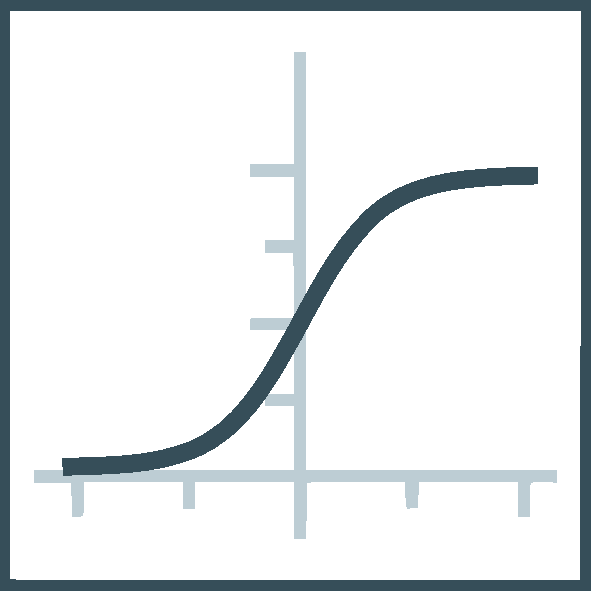
\includegraphics[height=3em]{images/sigmoid.pdf}\end{figure}
	\end{minipage}%
	\vspace{2em}
	Poly-Phen2\\{\tiny\parencite{Adzhubei2010}}
	}
	}
	child {%
	node {%
	\begin{minipage}{.6\textwidth}%
		Machine learning
	\end{minipage}%
	\begin{minipage}{.4\textwidth}%
		\begin{figure}
\includegraphics[height=3em]{images/ai.pdf}\end{figure}
	\end{minipage}%
	\vspace{2em}
	SNAP2\\{\tiny\parencite{Hecht2015}}\\\vspace{1ex}Envision\\{\tiny\parencite{Gray2018}}
	}
	}
	}
	child {%
	node {Unsupervised}[sibling distance=8em, level distance=8em]
	child {%
	node {%
	\begin{minipage}{.6\textwidth}%
		Statistical model
	\end{minipage}%
	\begin{minipage}{.4\textwidth}%
		\begin{figure}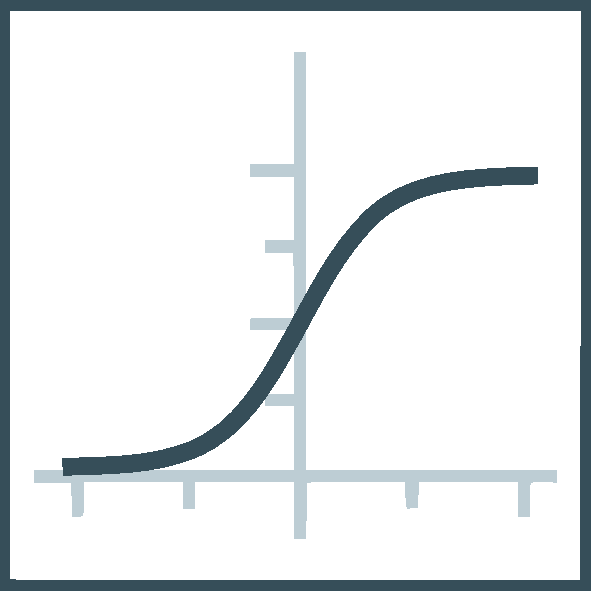
\includegraphics[height=3em]{images/sigmoid.pdf}\end{figure}
	\end{minipage}%
	\vspace{2em}
	EVmutation\\{\tiny\parencite{Hopf2017}}\\\vspace{1ex}SIFT\\{\tiny\parencite{Sim2012}}}
	}
	child {%
	node {%
	\begin{minipage}{.6\textwidth}%
		Machine learning
	\end{minipage}%
	\begin{minipage}{.4\textwidth}%
		\begin{figure}
\includegraphics[height=3em]{images/ai.pdf}\end{figure}
	\end{minipage}%
	\vspace{2em}
	DeepSequence\\{\tiny\parencite{Riesselman2018}
	}
	}
	}
	};
\end{tikzpicture}%
